

%% La classe stageM2R s'appuie sur la classe memoir, plus d'information sur le paquet: http://www.ctan.org/pkg/memoir
%% option possible de la classe stageM2R
% utf8  -> encodage du texte UTF8 (défaut: Latin1)
% final -> mode rapport de stage final (défaut: mode étude bibliographique)
% private -> indique une soutenance privée (défaut: soutenance publique)
\documentclass[utf8]{stageM2R} %-> etude bibliographique
%\documentclass[utf8,final]{stageM2R} %-> rapport final

\usepackage[style=numeric,citestyle=numeric,backend=bibtex]{biblatex}
\usepackage{wrapfig}

\bibliography{../../articles/biblio.bib}

\newcommand*{\addheight}[2][.5ex]{%
  \raisebox{0pt}[\dimexpr\height+(#1)\relax]{#2}%
}

%%%%%%%%%%%%%%%%%%%%%%%%%%%%
%%% Déclaration du stage %%%
%%%%%%%%%%%%%%%%%%%%%%%%%%%%

%% auteur
\author{Noé Le Philippe}
%% encadrants
\supervisors{William Puech}
%% lieu du stage (Optionnel)
\location{Équipe ICAR - LIRMM UM5506 - CNRS, Université de Montpellier}
%% titre du stage
\title{La phylogénie des images dans les réseaux sociaux} 
%% parcours du master
\track{IMAGINA}  
%% date de soutenance (Optionnel)
\date{\today} 
%% version du rapport (Optionnel)
\version{1}
%% Résumé en francais
\abstractfr{
Ce stage de master.
}
%% Résumé en anglais
\abstracteng{
  This master thesis.
}



\begin{document}   
%\selectlanguage{english} %% --> turn the document into english mode (Default is french)
\selectlanguage{french} 
\frontmatter  %% -> pas de numérotation numérique
\maketitle    %% -> création de la page de garde et des résumés
\cleardoublepage   
\tableofcontents %% -> table des matières
\mainmatter  %% -> numérotation numérique


%%%%%%%%%%%%%%%%%%%%%%%%%%%%%%
%%%%   DEBUT DU RAPPORT   %%%%
%%%%%%%%%%%%%%%%%%%%%%%%%%%%%%

\chapter{Introduction}
La phylogénie, en sciences naturelles, est définie\cite{phylogeny} comme l'étude des relations de parenté entre êtres vivants. Et c'est exactement de cela qu'il s'agit dans le cas des images, l'étude des relations de parenté entre images. \\
À l'ère des réseaux sociaux, il n'a jamais été aussi simple de partager des idées et du contenu. À chaque partage cependant, l'information peut être amenée à être modifiée. Les images, puisque c'est là notre sujet d'étude, peuvent avoir subi un certain nombre de transformations et modifications avant de nous parvenir. C'est dans ce contexte que nous allons intervenir, et tenter de reconstituer la phylogénie de l'image. Il peut être difficile de différentier cette image de l'originale, et de savoir laquelle est l'originale, mais c'est pourtant crucial dans un monde où l'information peut être falsifiée par tout le monde et extrêmement facilement. Les applications sont variées, et ne se cantonnent pas à la détection et la discrimination d'images altérées, on peut également se servir de la phylogénie de l'image pour optimiser de l'espace de stockage en ne gardant que l'originale ou encore suivre la diffusion et l'évolution des idées sur les réseaux sociaux.
\newpage

\subsection{Near-duplicate images (NDI)}
\label{subsec:ndi}
Nous travaillons sur un ensemble d'images, toutes similaires, et au milieu de cette jungle d'images, nous devons décider quelle image est le parent de quelle autre, ou autrement dit, quelles images sont des \textbf{near-duplicates}. Joly et al. \cite{joly2007content} définit la notion de near-duplicate comme suit : $I_{1} = T(I), T \in \mathcal{T}$ où $I$ est l'image parent, $I_{1}$ est l'image enfant et $\mathcal{T}$ est un ensemble de transformations autorisées, $I_{1}$ et $I$ sont alors des NDI. Dans le cas général, $\mathcal{T} = $ \textit{\{resampling, cropping, affine warping, color changing, lossy compression\}}, Fig. \ref{fig:near-duplicates-images} montre un exemple de near-duplicates, dans le cadre de ce stage cependant, $\mathcal{T} = $ \textit{\{lossy compression\}}. Notons l'utilisations du terme \textit{transformations autorisées}. Ce terme est double, d'une part, il place une limite arbitraire dans la force de la transformation, par exemple une image cropée à plus de 10\% pourra ne pas pas être considérée comme un near-duplicate, et d'autre part, il permet de restreindre l'espace des transformations possibles. Ainsi, dans le cadre du stage, seules les images de la troisième case de Fig. \ref{fig:near-duplicates-images} seront des NDI. Ces transformations peuvent évidemment se composer, et une image enfant peut être le résultat de plusieurs transformations.

\begin{figure}
\begin{center}
\begin{tabular}{|c|c|c|}
      \hline
      \addheight{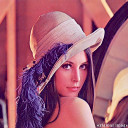
\includegraphics[width=23mm]{images/lena_base.jpg} 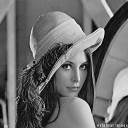
\includegraphics[width=23mm]{images/lena_bw.jpg}} &
      \addheight{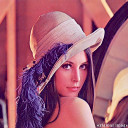
\includegraphics[width=23mm]{images/lena_base.jpg} 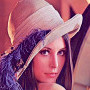
\includegraphics[width=23mm]{images/lena_crop.jpg}} &
      \addheight{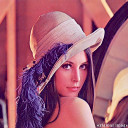
\includegraphics[width=23mm]{images/lena_base.jpg} 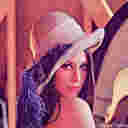
\includegraphics[width=23mm]{images/lena_comp.jpg}} \\
      \small couleur $\to$ noir et blanc & image entière $\to$ crop & image $\to$ image compressée\\
      \hline
\end{tabular}
\label{fig:near-duplicates-images}
\caption{Exemples de near-duplicates}
\end{center}
\end{figure}

\subsection{Arbre phylogénétique (Image Phylogeny Tree - IPT)}
C'est l'arbre représentant les relations de parenté entre les différentes images. Il sera extrait d'un ensemble de NDI, c'est l'objectif final de l'application. Un exemple est disponible Fig. \ref{fig:set_to_tree}. Le passage d'une génération à l'autre, autrement dit d'un noeud à son fils se fait à travers la transformation $I_{1} = T(I)$, ainsi, une image et son parent sont des NDI, alors qu'une images et ses soeurs ne le sont pas (Fig \ref{fig:tree_extract}).
\\ \indent
La reconstruction de l'arbre se concentre autour de deux problèmes principaux. Le premier est l'identification de la racine, et le second et l'estimation du reste de l'arbre. Il est en effet critique d'identifier correctement la racine. Prenons par exemple un des cas d'utilisation de l'IPT, la détection d'altération d'images. L'idée est que pour un ensemble d'images, plus on est proche de la racine, moins l'image a subi de transformations, et donc moins elle est altérée, avec dans le meilleur des cas, la racine en image originale. On voit bien que si on identifie mal la racine, on déduira, à tort, qu'une image n'a pas été altérée. Il n'est pas toujours garanti que la totalité des images de l'arbre original soit présente, de plus, certaines transformations peuvent être mineures, et difficile à détecter, c'est donc bien une estimation de l'arbre original qui sera faite.

\begin{figure}
  \begin{center}
    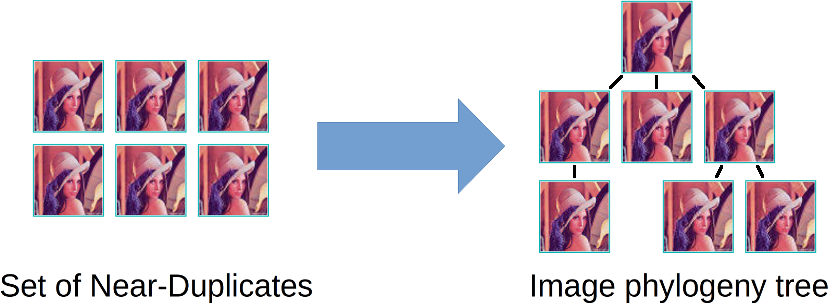
\includegraphics[width=120mm]{images/set_to_tree}
    \caption{Passage d'un ensemble de NDI à un arbre phylogénétique}
    \label{fig:set_to_tree}
  \end{center}
\end{figure}

\begin{figure}
  \begin{center}
    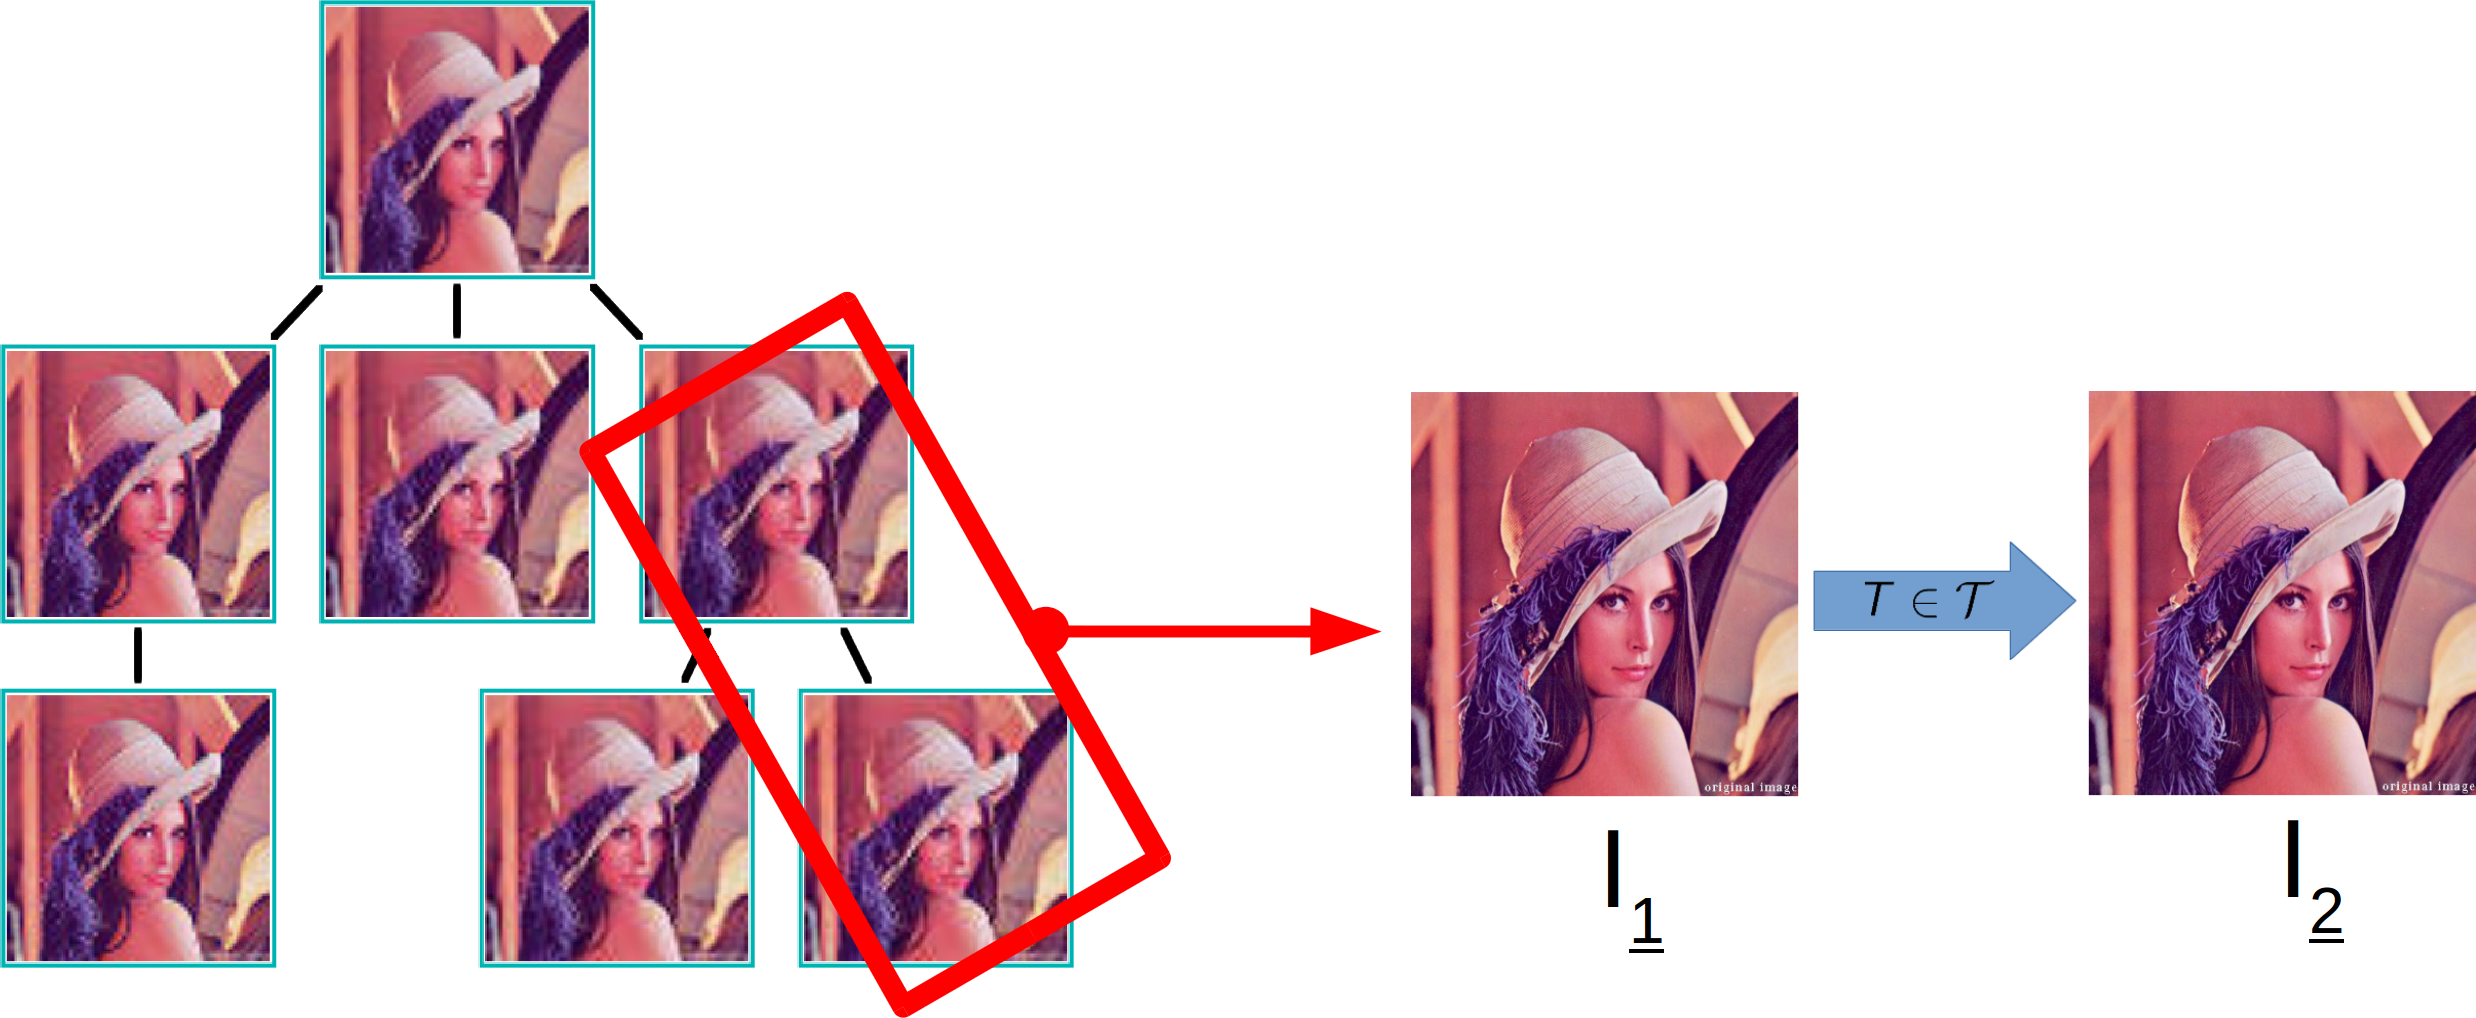
\includegraphics[width=120mm]{images/tree_extract}
    \caption{Passage d'une image parent à l'image enfant}
    \label{fig:tree_extract}
  \end{center}
\end{figure}

\subsection{Pourquoi se restreindre à la compression ?}
Comme mentionné précédemment, nous ne considérons que le cas de la compression avec perte en laissant de coté les autres transformations. Nous avons décidé de ne nous concentrer que sur une seule transformation pour avoir la possibilité de la traiter en détail et en profondeur dans le cadre du stage et ne pas devoir survoler sans approfondir toutes les transformations. Le choix de la compression est assez naturel, cela n'a, à notre connaissance, pas encore été traité dans le cadre le la phylogénie, et c'est un domaine largement étudié en forensic.

\chapter{État de l'art}
\section{État de l'art - Étude de l'arbre phylogénétique}
C'est un sujet qui, ces dernières années, n'a retenu l'attention que de deux équipes de recherche, nous allons ici présenter leurs travaux.
\subsection{La Visual Migration Map (VMM)}
C'est à notre connaissance, le premier article concernant vraiment notre sujet. Kennedy et al. \cite{kennedy2008internet} proposent une approche permettant d'automatiquement détecter la manière dont une image a été éditée ou manipulée, et d'en extraire des relations parent-enfant entre les images. Il vont construire à partir le l'estimation de ces transformations une Visual Migration Map (VMM) (voir Fig. \ref{vmm}) qui est en fait notre arbre de phylogénie.
\\ \indent
Ils partent du principe que les transformations sont directionnelles, c'est à dire que l'on de ne peut passer que d'une image moins transformée à une image plus transformée. Ainsi, ils vont tenter d'estimer la direction de chaque transformation entre deux images $I_{1}$ et $I_{2}$ (sachant que $\mathcal{T}$ = \textit{\{scaling, cropping, grayscale, overlay, insertion\}}). Trois scénarios sont alors possibles : si toutes des transformations sont dans le même sens, l'image fille est alors celle vers qui pointent les transformations, si les transformations sont dans des sens contraires, les images sont surement des soeurs, elles n'ont ent tous cas pas de relation parent-enfant, et enfin si aucune transformation n'a été détectée, c'est que soit les images sont identiques, soit elles ne sont pas des near-duplicates. On peut en voir un exemple Fig. \ref{vmm_directionnel}.
\\ \indent
Un graphe va ensuite être construit à partir des couples d'images pour lesquels une relation parent-enfant a été détectée. À noter qu'une relation parent-enfant ne veut pas forcément dire que c'est le parent direct mais plutôt un ancêtre. Ainsi, un noeud du graphe (une image) peut avoir plusieurs noeuds parents, pour finalement obtenir l'arbre désiré, seuls les chemins les plus longs sont conservés, comme on peut le voir Fig. \ref{vmm_tree}.

%%%%% parler de comment sont calculés les directions des transformations.
%%%%% parler des résultats ?
%%%%% parler de ce qui est bien dans cette méthode et de ce que l'on va utiliser.

% \begin{wrapfigure}{R}{0.5\textwidth}
%   \begin{center}
%     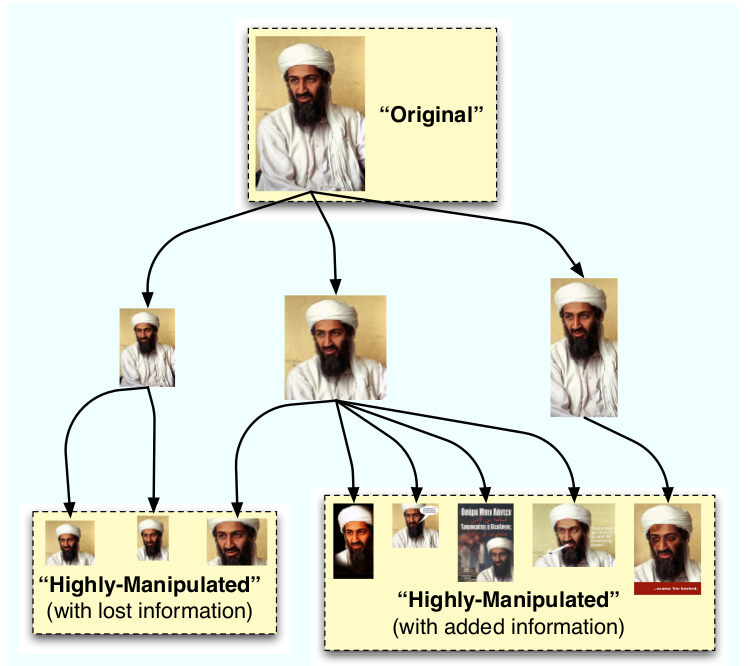
\includegraphics[width=0.48\textwidth]{images/vmm.png}
%   \end{center}
%     \label{vmm}
%     \caption{Exemple de VMM, tiré de \cite{internet}}
% \end{wrapfigure}

\begin{figure}
  \begin{center}
    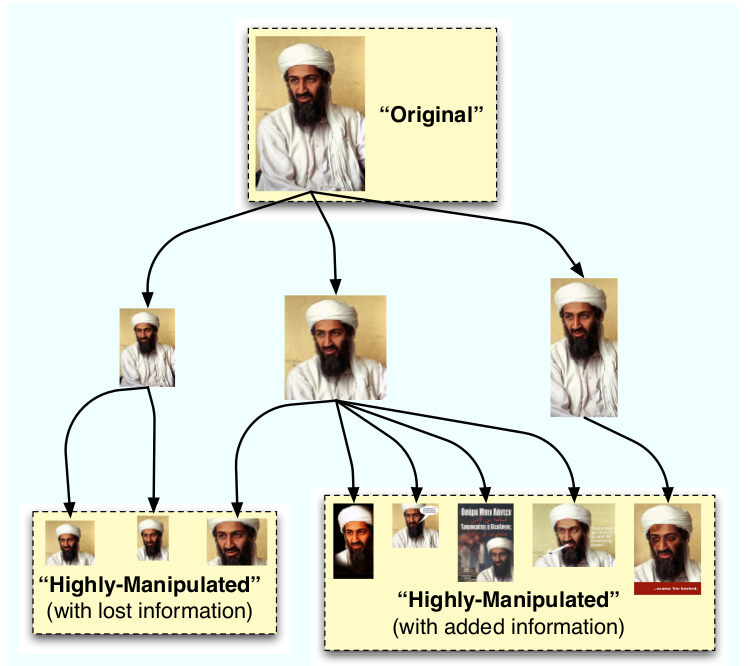
\includegraphics[width=70mm]{images/vmm.png}
    \label{vmm}
    \caption{Exemple de VMM, issu de \cite{kennedy2008internet}}
  \end{center}
\end{figure}

\begin{figure}
  \begin{center}
    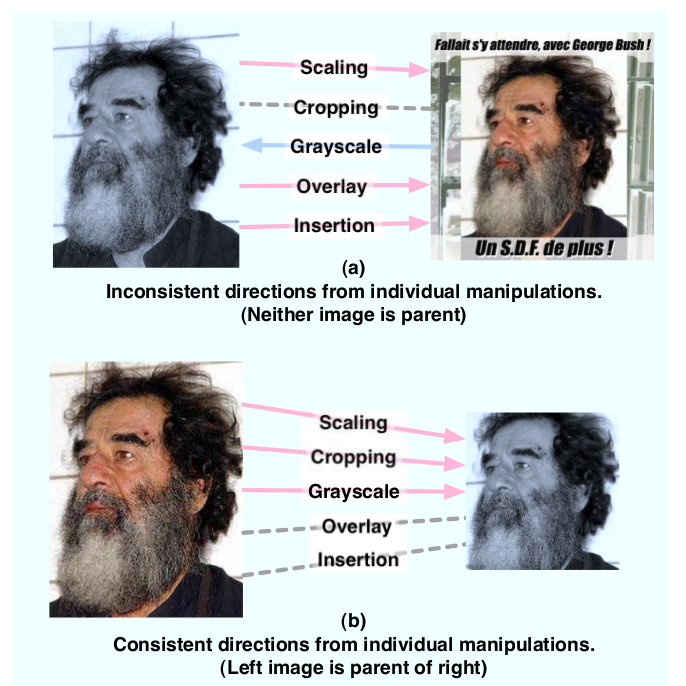
\includegraphics[width=70mm]{images/vmm_directionnel.png}
    \label{vmm_directionnel}
    \caption{Exemple de direction des transformations, issu de \cite{kennedy2008internet}}
  \end{center}
\end{figure}

\begin{figure}
  \begin{center}
    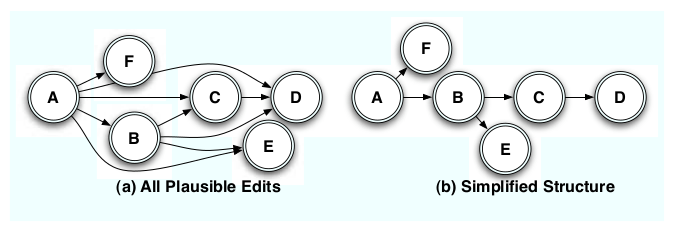
\includegraphics[width=100mm]{images/vmm_tree.png}
    \label{vmm_tree}
    \caption{Exemple de simplification de graphe, issu de \cite{kennedy2008internet}}
  \end{center}
\end{figure}

\subsection{Image Phylogeny Tree (IPT)}

\section{État de l'art - Analyse des recompression JPEG}

\chapter{Notre approche}

\chapter*{Conclusion}

\printbibliography

\end{document}

    
%%% Local Variables: 
%%% mode: latex
%%% TeX-master: t
%%% End:  
 